\documentclass[12pt,a4paper,oneside,titlepage]{article}
\usepackage[authoryear,longnamesfirst,round, comma]{natbib}               %Zitieren
\usepackage{graphicx}             %Graphik-Paket
\usepackage{color}
\usepackage[USenglish]{babel}     %Spracheinstellung USEnglish
\usepackage[utf8]{inputenc}       %Umlaute & Akzente
\usepackage{lmodern}              %Computer-Modern als Vektorgrafiken

\usepackage{setspace}             %Zeilenabstand 1,5
\onehalfspacing
%Zeilenabstand vor und nach Gleichungen ändern
\makeatletter
\g@addto@macro\normalsize{%
  \setlength\abovedisplayskip{2pt}
  \setlength\belowdisplayskip{5pt}
  \setlength\abovedisplayshortskip{0pt}
  \setlength\belowdisplayshortskip{0pt}
}
\makeatother

\usepackage{geometry}             %Seitenränder anpassen
\geometry{a4paper,left=30mm,right=25mm, top=2cm, bottom=3cm}



\usepackage{microtype}            %besseres Schriftbild
\usepackage{footmisc}             %Fußnoten

\usepackage[tbtags]{mathtools}            %Mathematische Symbole
\usepackage{amsmath, amsthm, amssymb, amsfonts}    %bessere mathematische Formeln

\usepackage{booktabs}             %bessere Tabellen
\usepackage{marvosym}             %Symbole einfügen


\usepackage{titletoc}			  %Inhaltsverzeichnis anpassen
\dottedcontents{section}[3em]{\bfseries}{2.9em}{1pc}
\dottedcontents{subsection}[4em]{}{3.3em}{1pc}

\usepackage[small]{titlesec}     %Überschriften anpassen

\usepackage{epstopdf}            %include Matlab Figures


\renewcommand{\thesection}{\Roman{section}}  %Römische Zahlen bei Überschrift
\renewcommand{\thesubsection}{\thesection.\Roman{subsection}}





\begin{document}
\parindent 0pt %kein Erstzeileneinzug
\begin{titlepage}
	\centering
	
\includegraphics[width=0.8\textwidth]{pictures/LogoFU}\par\vspace{1cm}
	{\scshape\large Freie Universität Berlin \par}
	\vspace{1cm}
	{\scshape\large Seminar Paper in "Recent Research in Macroeconomics"\par}
	\vspace{1.5cm}
	{\LARGE\bfseries Reimplementation of Erceg \& Lindé (2012):\par}
	\vspace{0.5cm}
	{\Large\bfseries Is there a Fiscal Free Lunch in a Liquidity Trap?\par}
	\vspace{2cm}
	{\Large\itshape Denis Maciel \& Tobias Müller\par}
	\vfill
	supervised by\par
	Prof. Dr. Mathias \textsc{Trabandt}

	\vfill

% Bottom of the page
	{\large \today\par}
\end{titlepage}


\doublespacing
\tableofcontents

\pagebreak[4]
\listoffigures
\listoftables
\newpage

\section{Introduction}

The financial crisis in 2008 and the following worldwide recession marked a turning point in the economic and public debate about optimal fiscal and monetary policy. In the aftermath of the great recession, economists discussed about the effects of an expansionary fiscal policy to stabilize the economy and stimulate the private sector. The focus of the analysis has been on the size of the fiscal multiplier and the rise of the output in response to a government spending hike.
\par
\bigskip
The economic crisis challenged the state of the art of the economic research at this time. To prevent the economy not to fall in a prolonged recession, governments and central banks launched unconventional and in part uncharted measures. When central banks reduced the interest rates down to the zero lower bound, fiscal policy became more important to counteract the deflationary spiral and the large output gap of the recession. The increasing literature about fiscal policy and the government spending multiplier, as well as new developments in general equilibrium models, suggest the effectiveness of government spending, when the nominal interest rate hits the zero lower bound. Normally, the fiscal multiplier is not only larger in an environment of a liquidity trap, but also comes together with minimal budgetary costs.
\par
\bigskip
Therefore, the authors Christopher Erceg and Jesper Lindé address in the paper \textit{"Is there a Fiscal Free Lunch in a liquidity trap?"} the question whether policymakers should limit the size of the government spending. As we will see in this paper, the distinction between marginal and average size of the fiscal multiplier is crucial for policymakers to better understand the effects of the implemented policies. The paper also gives new insights on how fiscal spending and austerity measures impact the government budget in a liquidity trap. The authors contribute with their paper to the current discussion about the efficient use of fiscal policy when monetary policy reaches its limit. By reimplementing the paper in Matlab \& Dynare, we followed the aims of the seminar to develop economic intuition and quantitative
methodological expertise, as well as the understanding of the current macroeconomic policy debates.
\par
\bigskip

Our paper is organized as follows. In Section II, we discuss briefly the current literature about the government spending multiplier and give the main results of the analyzed paper. In Section III, we concentrate on the key equations of the paper, explain the structure of the model and exemplify the interpretation of the shock parameters. In Section IV, we present the results of the impulse responses to show how the model reacts to an exogenous consumption taste shock and government-spending shock. We also give some impressions on how the results vary if we change the parameters of the monetary rule and the slope of the Phillips curve. In Section V, we develop the concept of the marginal and average fiscal multiplier. We show that the variation of the fiscal multiplier depends highly on the size of the government response and the price contract duration. In Section VI, we analyze the impacts of the government spending on the budget. In Section VII we provide some additional information on our work-flow. We conclude our paper with the main takeaways and a short critique.


\section{Fiscal Policy and the Spending Multiplier }

new evidence on recent model-based economic research raised the question whether fiscal policy can be an adequate response in a deep and prolonged recession.
- NK framework

The impacts of higher spending or fiscal consolation measures in an environment of a liquidity trap when the nominal interest rate hits zero,

Fiscal policy can play a crucial role in stabilizing the economy during an economic crisis. Recent literature shows that the government spending multiplier is particularly large in recessions. Improvements in the economic research and new developments in New Keynesian Model literature after the financial crisis 2008 can help the political decision makers to better understand optimal policies in times of an great economic downturn. Eggertsson (2008), David and Leeper (2011) and Christiano, Eichenbaum and Rebelo (2011) show that an increase in government spending can outsize the effect on output in a deep recession. Especially in prolonged liquidity traps, there can be a strong case for a fiscal stimulus on a temporary basis to jump start the economy and push it out of an economic downward spiral.
The key question of the paper "Is there a fiscal free lunch in a liquidity trap" concentrates on the magnitude of the government spending multiplier under different frameworks and the impact of the fiscal policy on the government budget.

  - Fiscal spending in a liquidity trap is very efficient
  - Multiplier is high but decreases quickly...
  - results depend highly on the framework of the model - we will show the level of price stickiness, monetary policy rule

\section{The Model}
In this section we describe and summarize the baseline illustration of the New Keynesian dynamic stochastic general equilibrium (DSGE) model \citet{Erceg.2014} use in their paper\footnote {Additional information and a more detailed derivation of the standard log-linearized version of the New Keynesian model can be found in the Online Appendix of the original paper.}. The New Keynesian DSGE model has a RBC-core, but allows two inefficiencies, so that shocks can cause deviations from the "natural level": monopolistic competition among firms and the Calvo model of firms' price setting. Therefore, the New Keynesian model addresses the deficits of the RBC-models and makes the more realistic assumptions that prices are not adjusted continuously and real world markets are not perfectly competitive. Consequently, monetary policy can affect the real interest rate, thus has real effects. The microfoundation allows a normative policy analysis. 
\subsection*{Households}

The representative household decides the intertemporal consumption demand by maximizing
\begin{equation}
E_t \sum_{j=0}^\infty \beta^j \left\{ \frac{1}{1- \frac{1}{\sigma}} \left(C_{t+j} - C\nu_{t+j}\right)^{1-\frac{1}{\sigma}} - \frac{N_{t+j}^{1+\chi}}{1+\chi} + \mu_0F \left(\frac{MB_{t+j+1}(h)}{P_{t+j}}\right)\right\} \nonumber
\end{equation}
under the constraint\newline
$P_t(1+\tau_{C,t})C_t + B_{G,t} + MB_{t+1} = (1-\tau_{N,t})W_tN_t + (1+i_{t-1})B_{G,t-1} + MB-T_t + \Gamma_t,$
where 0 $< \beta > 1$ is the discount factor and $E_t$ the rational expectations operator. The utility function depends on the households current consumption $C_t$ as deviation from a “reference level” $C\nu_{t+j}$, where C is steady state consumption, and a negative taste shock $\nu_t$ which reduces this reference level.
WICHTIG HIER CONSUMPTION TASTE SHOCK ERKLÄREN!
The utility function also depends inversely on hours worked $N_t$. The inclusion of money, as a zero nominal interest asset, provides a rationale for the zero lower bound on nominal interest rates. By assuming that $\mu_0$ is arbitrarily small, changes in real money balances have negligible implications for seignorage in the model. The households budget constraint implies that the expenditure on goods and net purchases of government bonds $B_{G,t}$ equals the after-tax labor income $ \left(1 - \tau_{N,t} \right) W_tN_t$, minus a lump-sum tax $T_t$, plus a proportional share of the profits $\Gamma_t$ of all intermediate firms. The households optimal plan needs to satisfy the first order condition, so that we receive
\begin{align}
\vspace{-0.5cm} \left(C_t - C\nu_t\right)^{-\frac{1}{\sigma}}  - \lambda_tP_t \left(1 + \tau_{C,t} \right) = 0,\nonumber\\
-N_t^{\chi} + \lambda_t \left(1 - \tau_{N,t} \right) W_t = 0,\nonumber\\
-\lambda_t + \beta \left(1 + i_t \right) E_t\lambda_{t+1} = 0,\nonumber
\end{align}
and finally the Euler equation
\begin{equation}
\frac {\left(C_t - C\nu_t\right)^{-\frac{1}{\sigma}}}{\left(1 + \tau_{C,t} \right)} = \beta E_t \frac{\left(1 + i_t \right)}{1 + \pi_{t+1}} \frac{\left(C_{t+1} - C\nu_{t+1}\right)^{-\frac{1}{\sigma}}}{\left(1+ \tau_{C,t+1}\right)},
\end{equation} 
and the aggregate labor supply relation
\begin{equation}
mrs_t \equiv \frac{N_t^\chi}{\left(C_t - C\nu_t\right)^{-\frac{1}{\sigma}}} = \frac{\left(1 - \tau_{N,t}\right)}{\left(1 + \tau_{C,t}\right)} \frac{W_t}{P_t}.
\end{equation}
The last equation shows that the marginal rate of substitution between consumption and labor must equal the real wage. 
We have to mention that in our simple New Keynesian Model we set the sales tax $\tau_{C,t}$ equal to zero, to get the same results as in the paper.

\subsection*{Firms}
The production function of the firms is
\begin{equation}
Y_t = K^\alpha N_t^{1-\alpha},\vspace{-0.3cm} \nonumber
\end{equation}
where aggregate capital is fixed, but shares of the aggregate capital stock can be allocated across the firms. All firms choose the factor demand such that costs are minimized. The real factor costs per marginal product therefore are
\begin{equation}
\frac{MC_t}{P_t} = \frac{W_t/P_t}{\left(1 - \alpha \right) K^\alpha N_t^{-\alpha}}.
\end{equation}
The firm, which can reset its price in period t, chooses a price $\left(P_t^{opt} \right)$ and maximizes the problem
\begin{equation}
\max_{P_t^{opt}\left(f\right)} E_t \sum_{j=0}^\infty \xi_p^j \psi_{t,t+j} \left[ \left(1 + \pi \right)^j P_t^{opt}\left(f\right) - MC_{t+j} \right] Y_{t+j} \left(f\right),\nonumber
\end{equation}
where $\psi_{t,t+j}$ is the discount factor and $\xi$ the probability that the firm's price set in t will still be valid in period t+1. The demand function for the good $\left(f\right)$ which faces the firm is given by 
\begin{equation}
Y_{t+j}\left(f\right) = \left[\frac{P_t \left(f\right)}{P_t} \right]^{\frac{-\left(1+\theta_p\right)}{\theta_p}} Y_t \nonumber,
\end{equation}
which varies with the relative price of the good, the substitution elasticity $\theta$ and the aggregate demand $Y_t$. The first order condition with optimal price $\left(P_t^{opt} \right)$ is
\begin{equation}
E_t \sum_{j=0}^\infty \xi_p^j \psi_{t,t+j} \left[ \frac{\left(1 + \pi \right)^j P_t^{opt}\left(f\right)}{1 + \theta_p} - MC_{t+j} \right] Y_{t+j}\left(f\right) = 0.
\end{equation}
For deriving the New Keynesian Phillips curve, we also need the average price of the final goods
\begin{equation}
P_t = \left[\left(1 - \xi_p\right)\left(P_t^{opt}\right)^{\frac{-1}{\theta_p}} + \xi_p \left(\left(1 + \pi\right)P_{t-1}\right)^{\frac{-1}{\theta_p}} \right]^{-\theta_p}.
\end{equation}
Finally, we have to derive the aggregate resource constraint
\begin{equation}
C_t + G_t \leq \left(\frac{P_t^*}{P_t}\right)^{\frac{\left(1+\theta_p\right)}{\theta_p}} K^\alpha N_t^{1-\alpha},
\end{equation}
where actual output $Y_t$ can be divided into private consumption and government spending $\left(Y_t \equiv C_t + G_t \right)$.

\subsection*{The Government}

\begin{equation}
B_{G,t} = \left(1 + i_{t-1}\right) + P_tG_t - \tau_{C,t}P_tC_t - \tau_{N,t}W_tN_t - T_t - MB_{t+1} + MB_t
\end{equation}


Monetary policy follows a Taylor rule, and
fiscal policy specifies that taxes respond to government debt.

By log-linearizing the equations (1) to (7) around the Steady State and some rearranging, we receive the key equations of the model used in the \citet{Erceg.2014} paper.

\section{Impulse Response}

The main steps to reimplicate the New Keynesian model the authors use are:
\begin{enumerate}
\item Write up the model equations in Dynare and set the correct parameter values\vspace{-0.3cm}
\item Solve the model without baseline shock and compute impulse to government spending and consumption taste shock\vspace{-0.3cm}
\item Impose zero lower bound on monetary policy and simulate simul effects of a large negative consumption demand shock so that the economy hits the zero lower bound\vspace{-0.3cm}
\item Get the right parameter and shock values for an eight quarter liquidity trap in an environment of an positive government spending shock equal to one percent of stead state output\vspace{-0.3cm}
\item Calculate the difference between the impulse responses of both shocks and the taste shock only to receive the effects of the government spending shock
\end{enumerate}

first try to rebuild figure 2
explaination of figure 2
role of real interest rate in NKM
Important cruxes to get the right results in the following 


\subsection*{The Shock Parameter}

observe first baseline shock and then both shocks

explanation of the values of the shock parameter

make sure that model hits the zero lower bound - find the right values for an 8 quarter liquidity trap

Calculate difference between both shocks and taste shock only to get the effects of the government shock only
the government shock only is 


\subsection*{The Calvo Price Setting}
set first inflation to zero
play around with calvo price setting
figure2 no inflation and figure 2 5 quarter contracts

Get Figure 1b

\subsection*{Policy rules}

change in monetary policy figure

Figure 1 a effects of fiscal policy on liquidity trap

Table 2 - diference values for taste shock (important to control values! :D)

Why is the fall in output so large when the economy hits the zero
bound? For a given fall in output, marginal cost falls and prices decline.
With staggered pricing, the drop in prices leads agents to expect future deflation. With the nominal interest rate stuck at zero, the real interest
rate rises. This perverse rise in the real interest rate leads to an increase
in desired saving, which partially undoes the effect of a given fall in
output. So, the total fall in output required to reduce desired saving to
zero is very large. (Christiano 2011)

\input{Multiplier}

\section{Impacts on the Government Debt}

\citet{Afonso.2010}
Critique government debt in financial crisis S.27/28

\section{Workflow}

%Screenshot Github



\section{Conclusion}

%Test

\citet{Erceg.2014}
\citet{Christiano.2011}\citet{CoenenG..2010}\citet{Erceg.2014}

\citet{Eggertsson.2011}
\citet{Coenen.2010}


\pagebreak[4]
\addcontentsline{toc}{section}{References}
\bibliographystyle{plainnat}  %Zitationsstil
\bibliography{References}


%Grafiken
\pagebreak[4]
\begin{figure}[th]
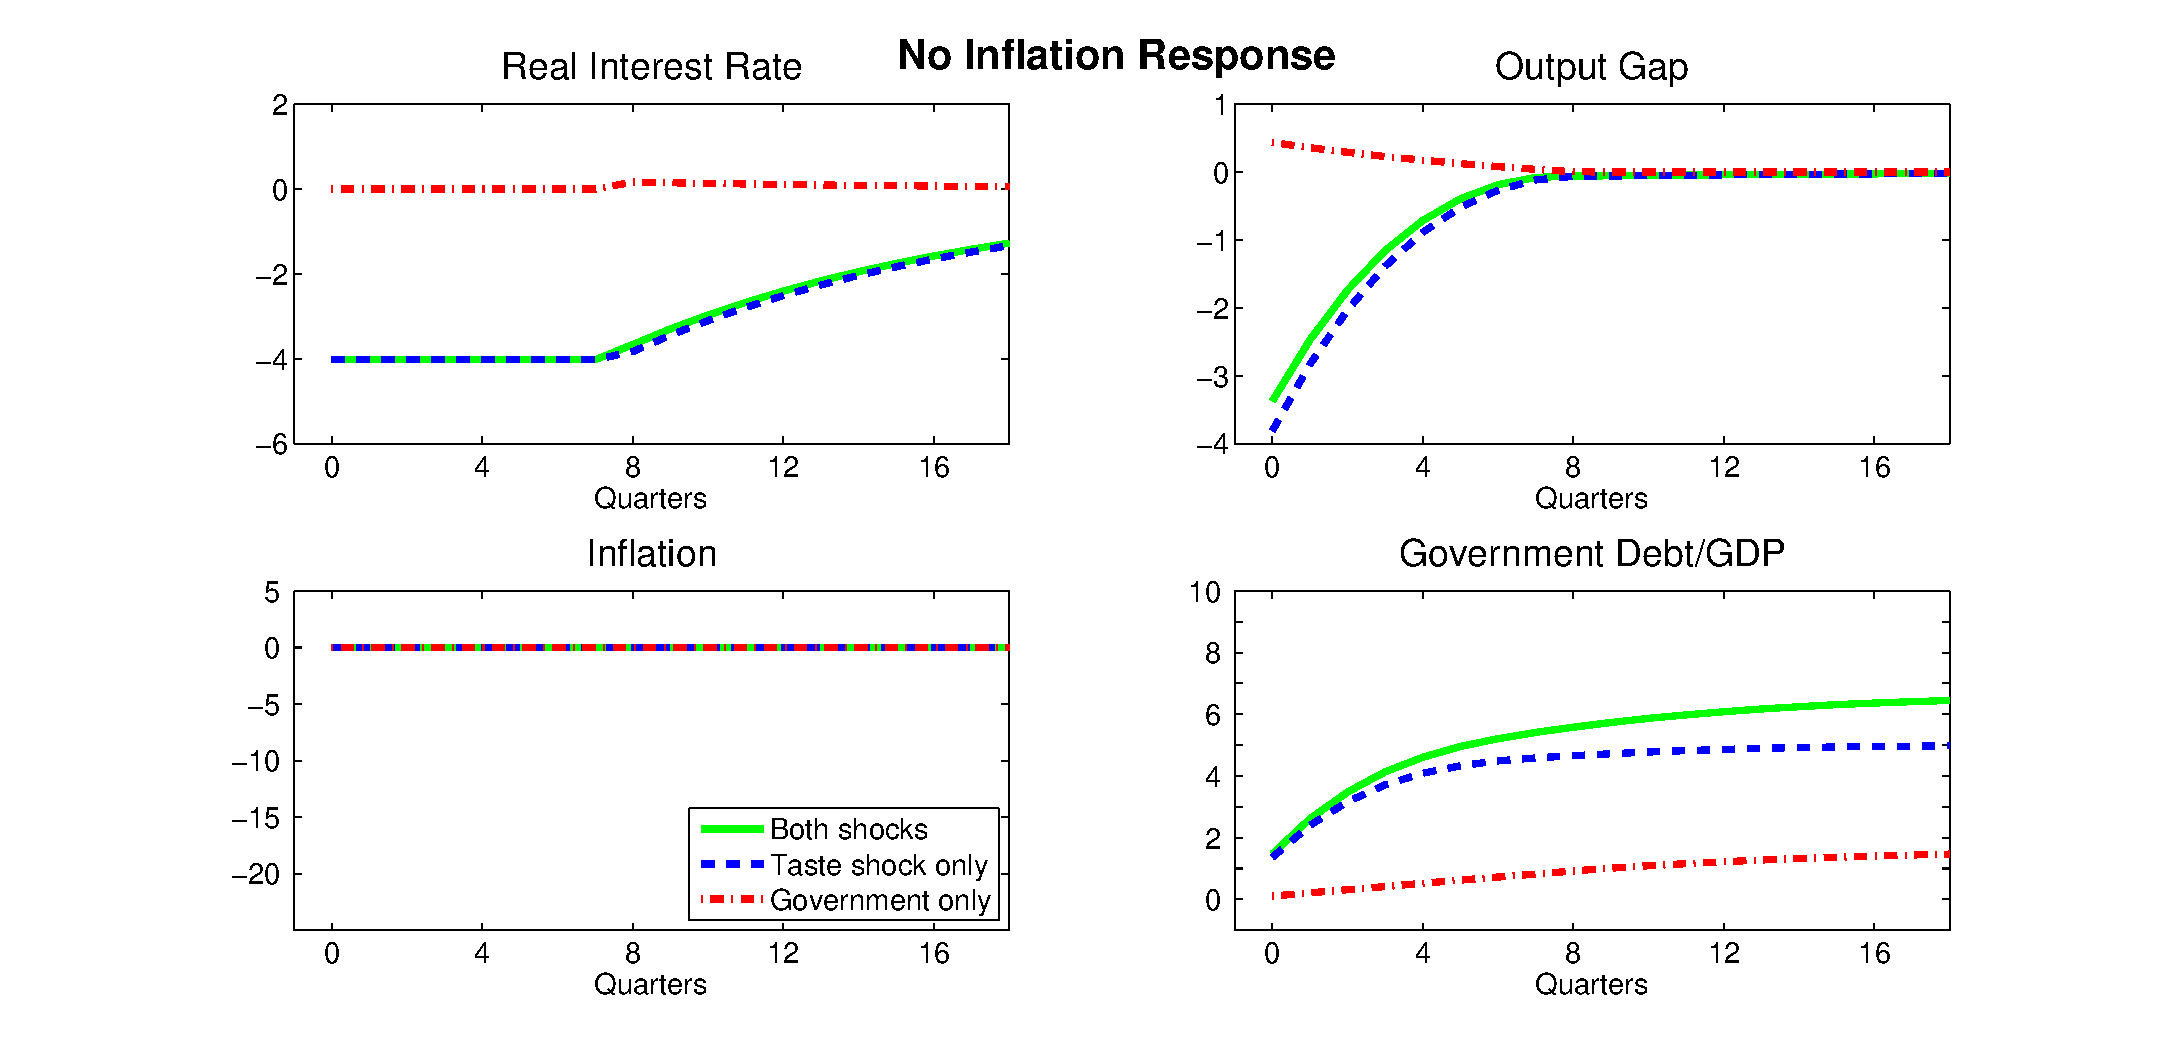
\includegraphics[width=\textwidth]{Paperpics/Figure2noIR}
\caption{Immediate Rise in Government Spending (No Inflation Response)}
\label{IRnoinflation}
\end{figure}
\vspace{2cm}

\begin{figure}[th]
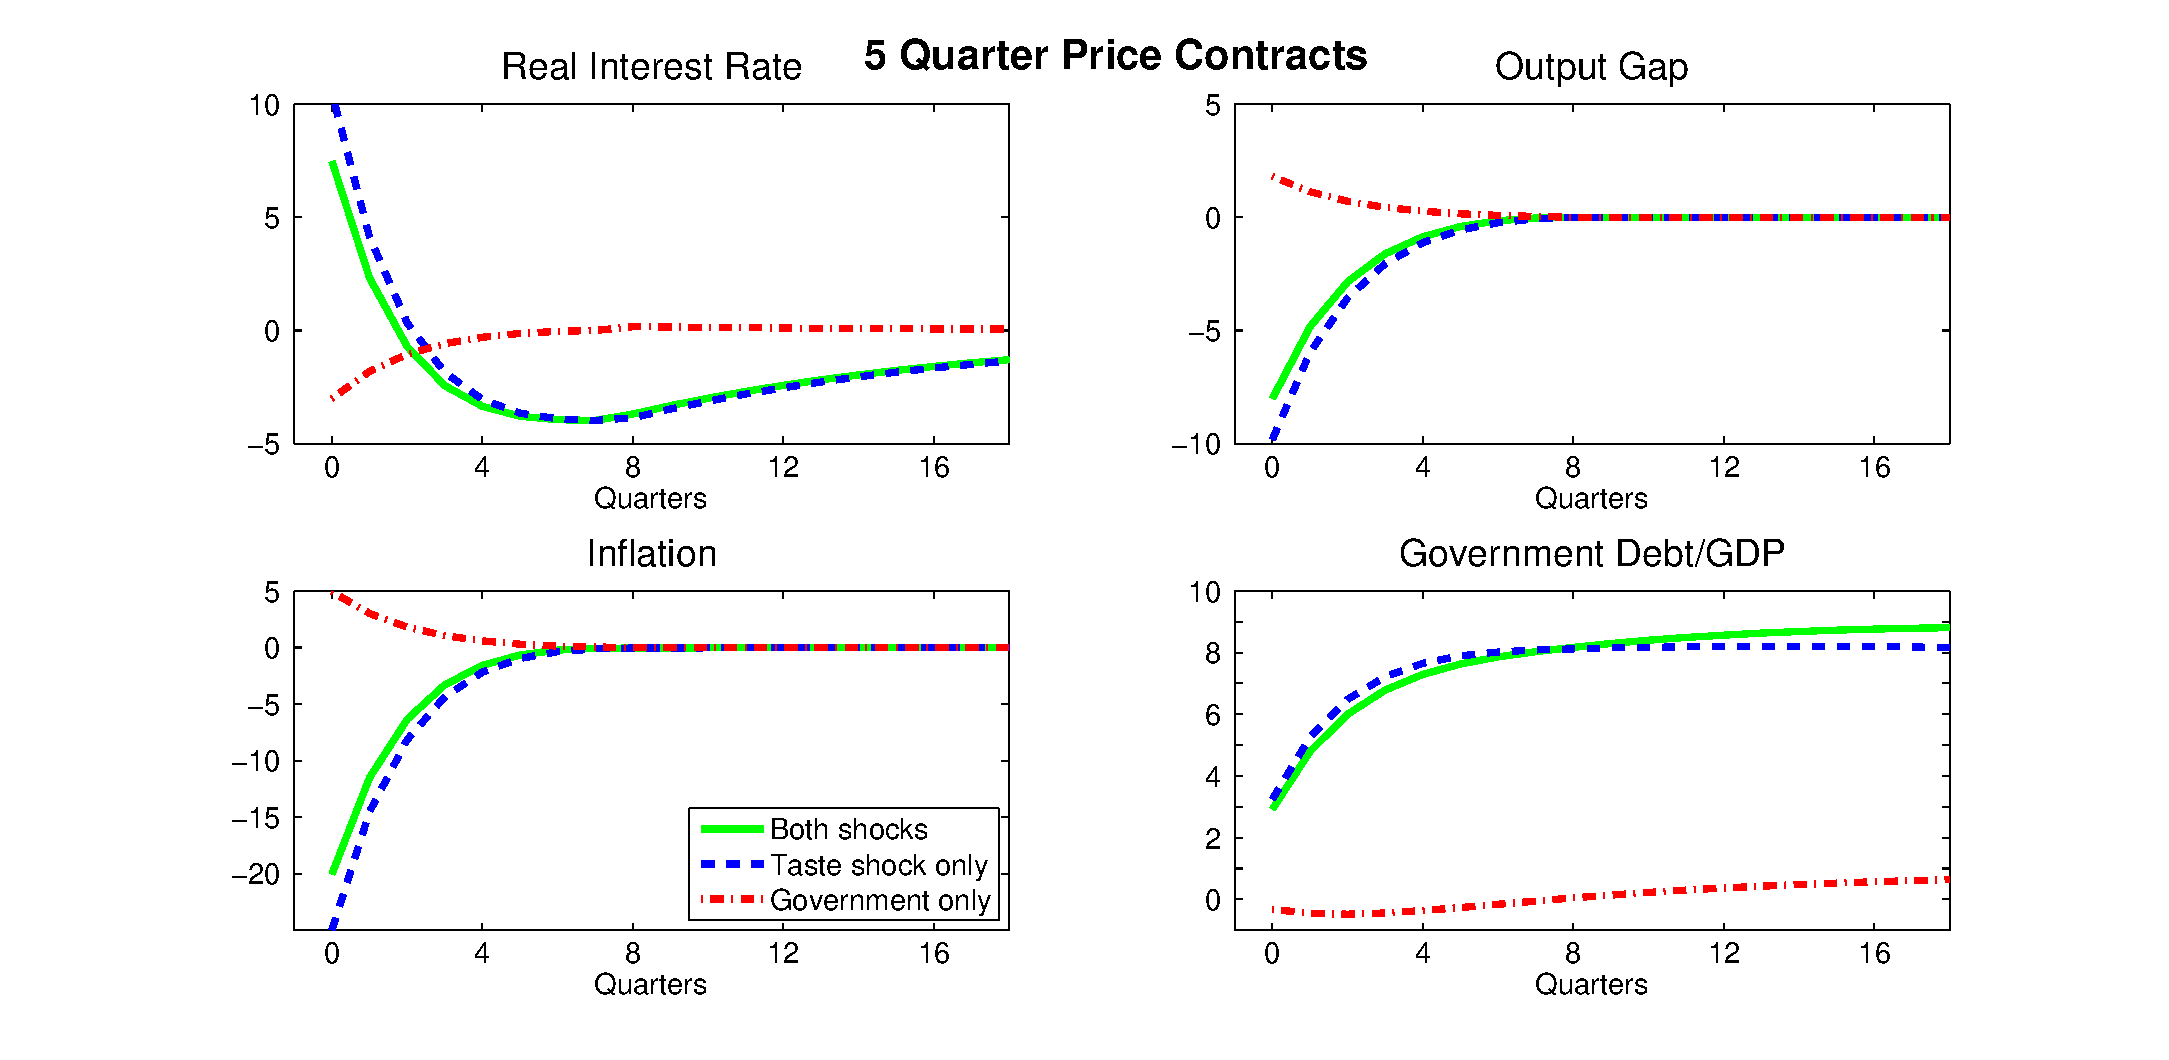
\includegraphics[width=\textwidth]{Paperpics/Figure25quarter}
\caption{Immediate Rise in Government Spending (5 Quarter Price Contracts)}
\label{IR5quarter}
\end{figure}
\bigskip

\begin{figure}[th]
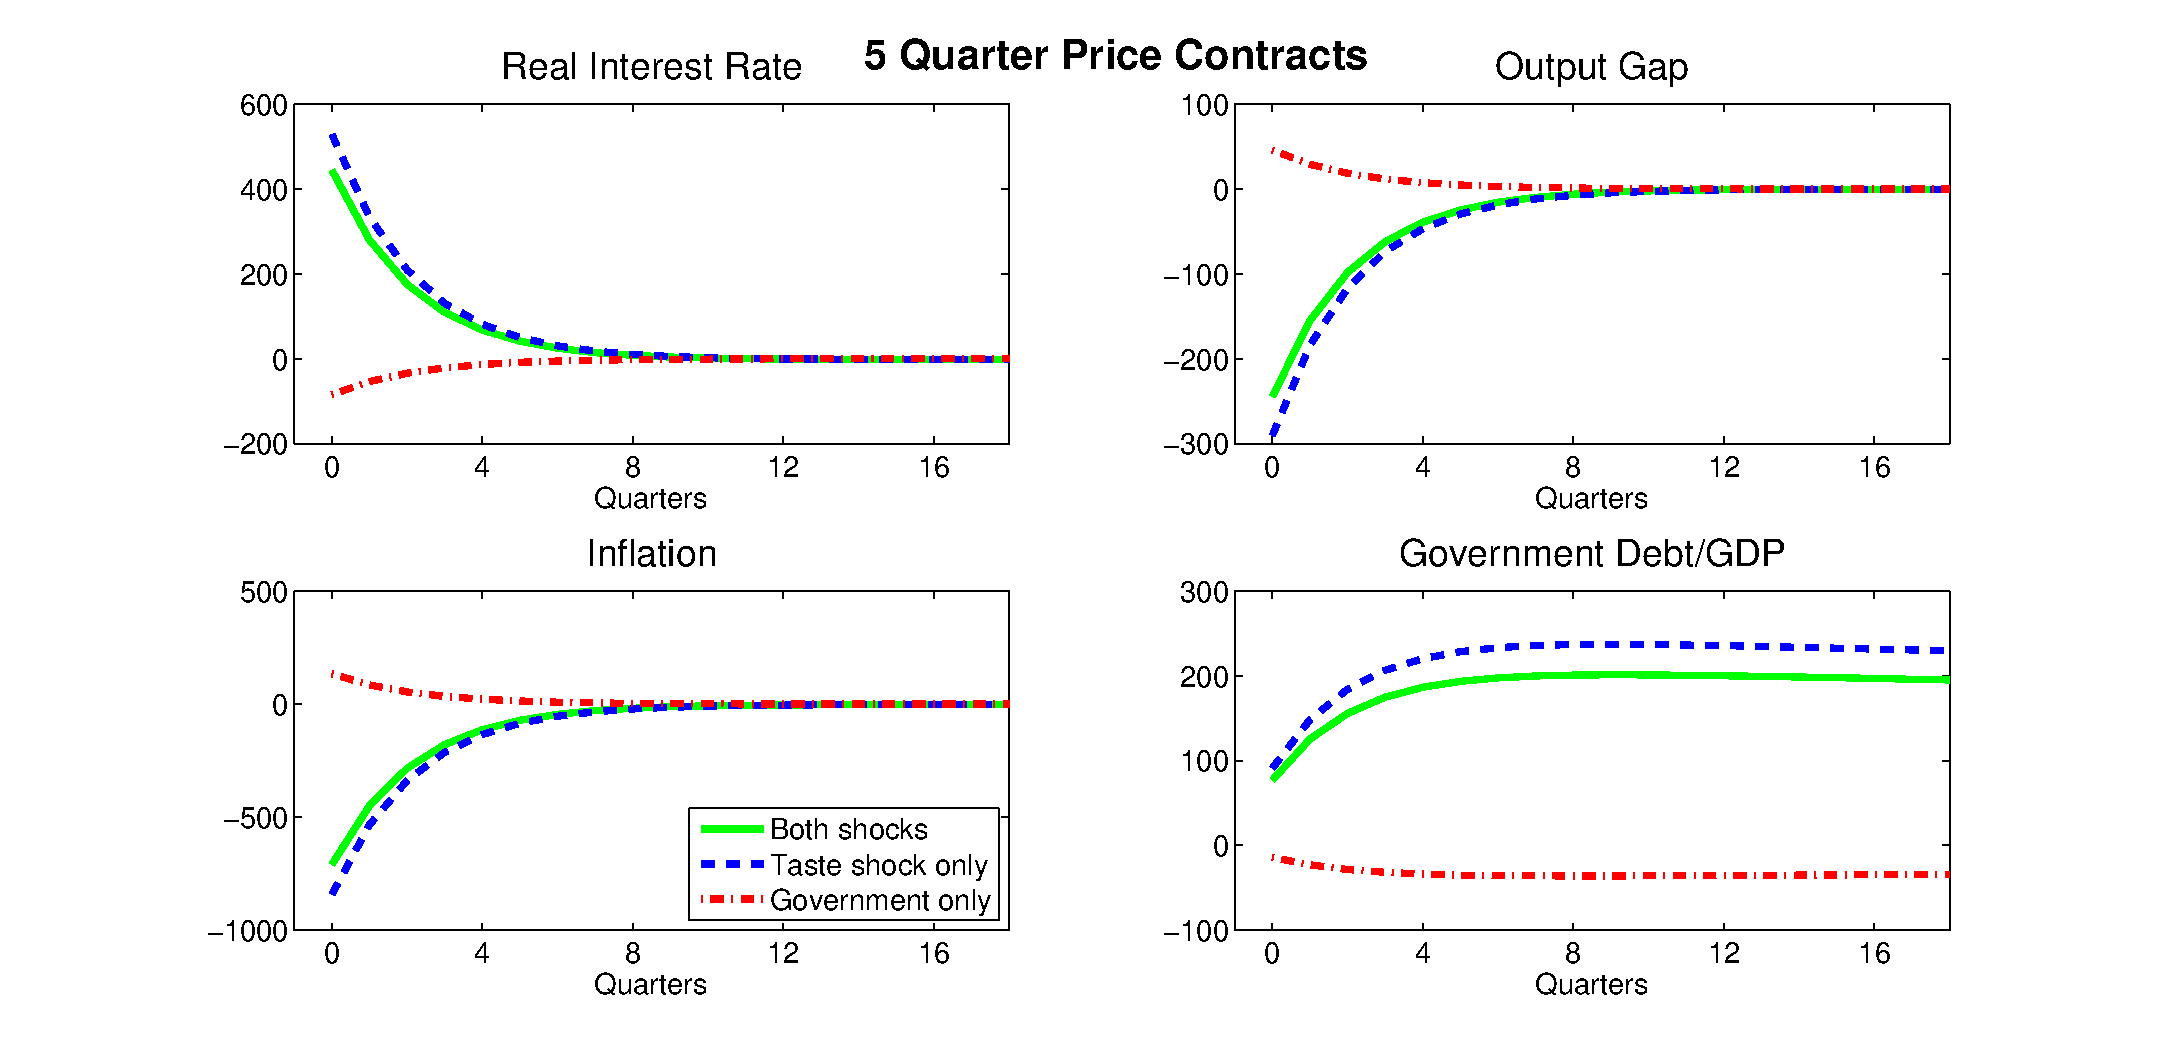
\includegraphics[width=\textwidth]{Paperpics/Figure25quarternewtaylorrule}
\caption{Immediate Rise in Government Spending (Alternative Taylor Rule Values)}
\label{IR5quarternewtr}
\end{figure}
\bigskip


\begin{figure}[th]
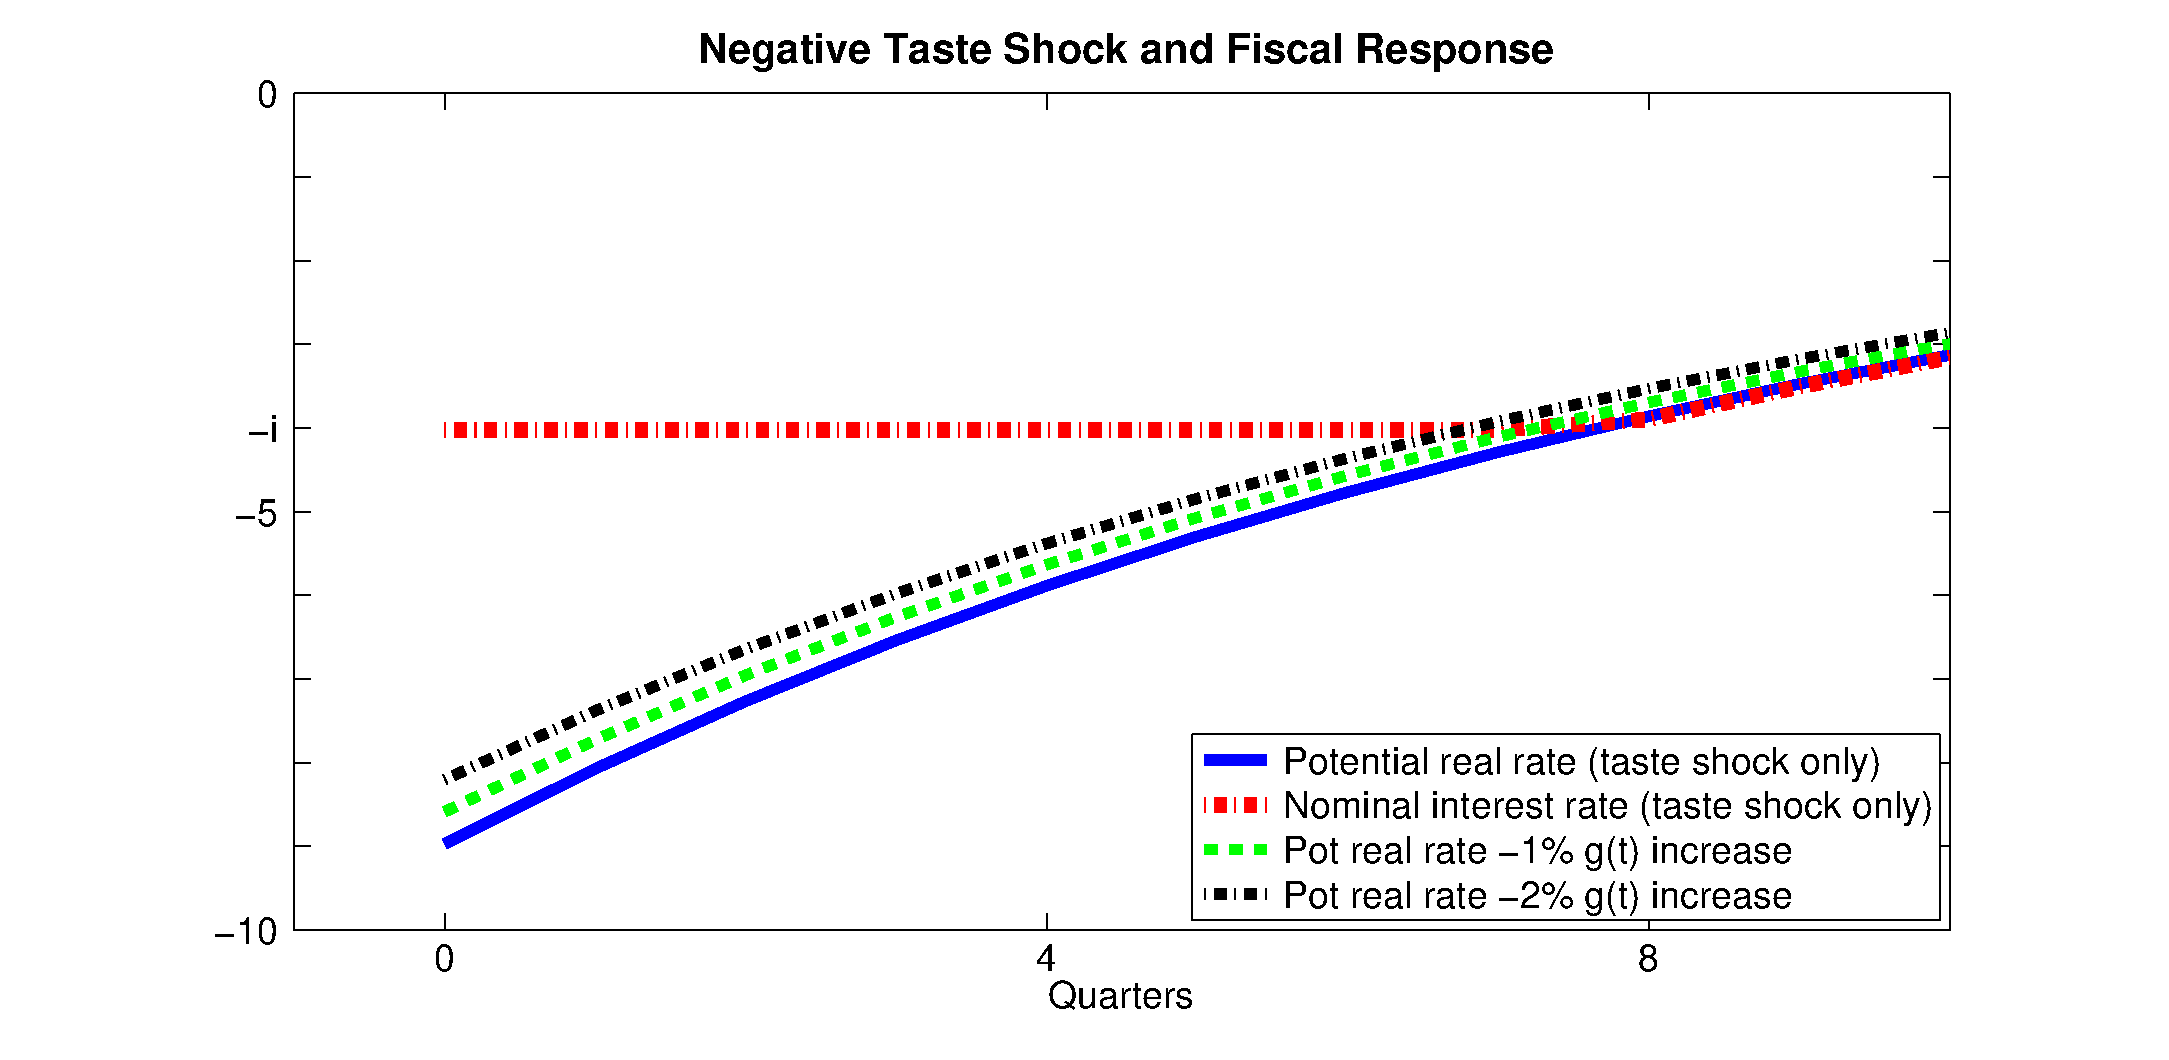
\includegraphics[width=\textwidth]{Paperpics/Figure1a}
\caption{Potential Real Interest Rate and Fiscal Response}
\label{Figure1a}
\end{figure}
\bigskip

\begin{figure}[th]
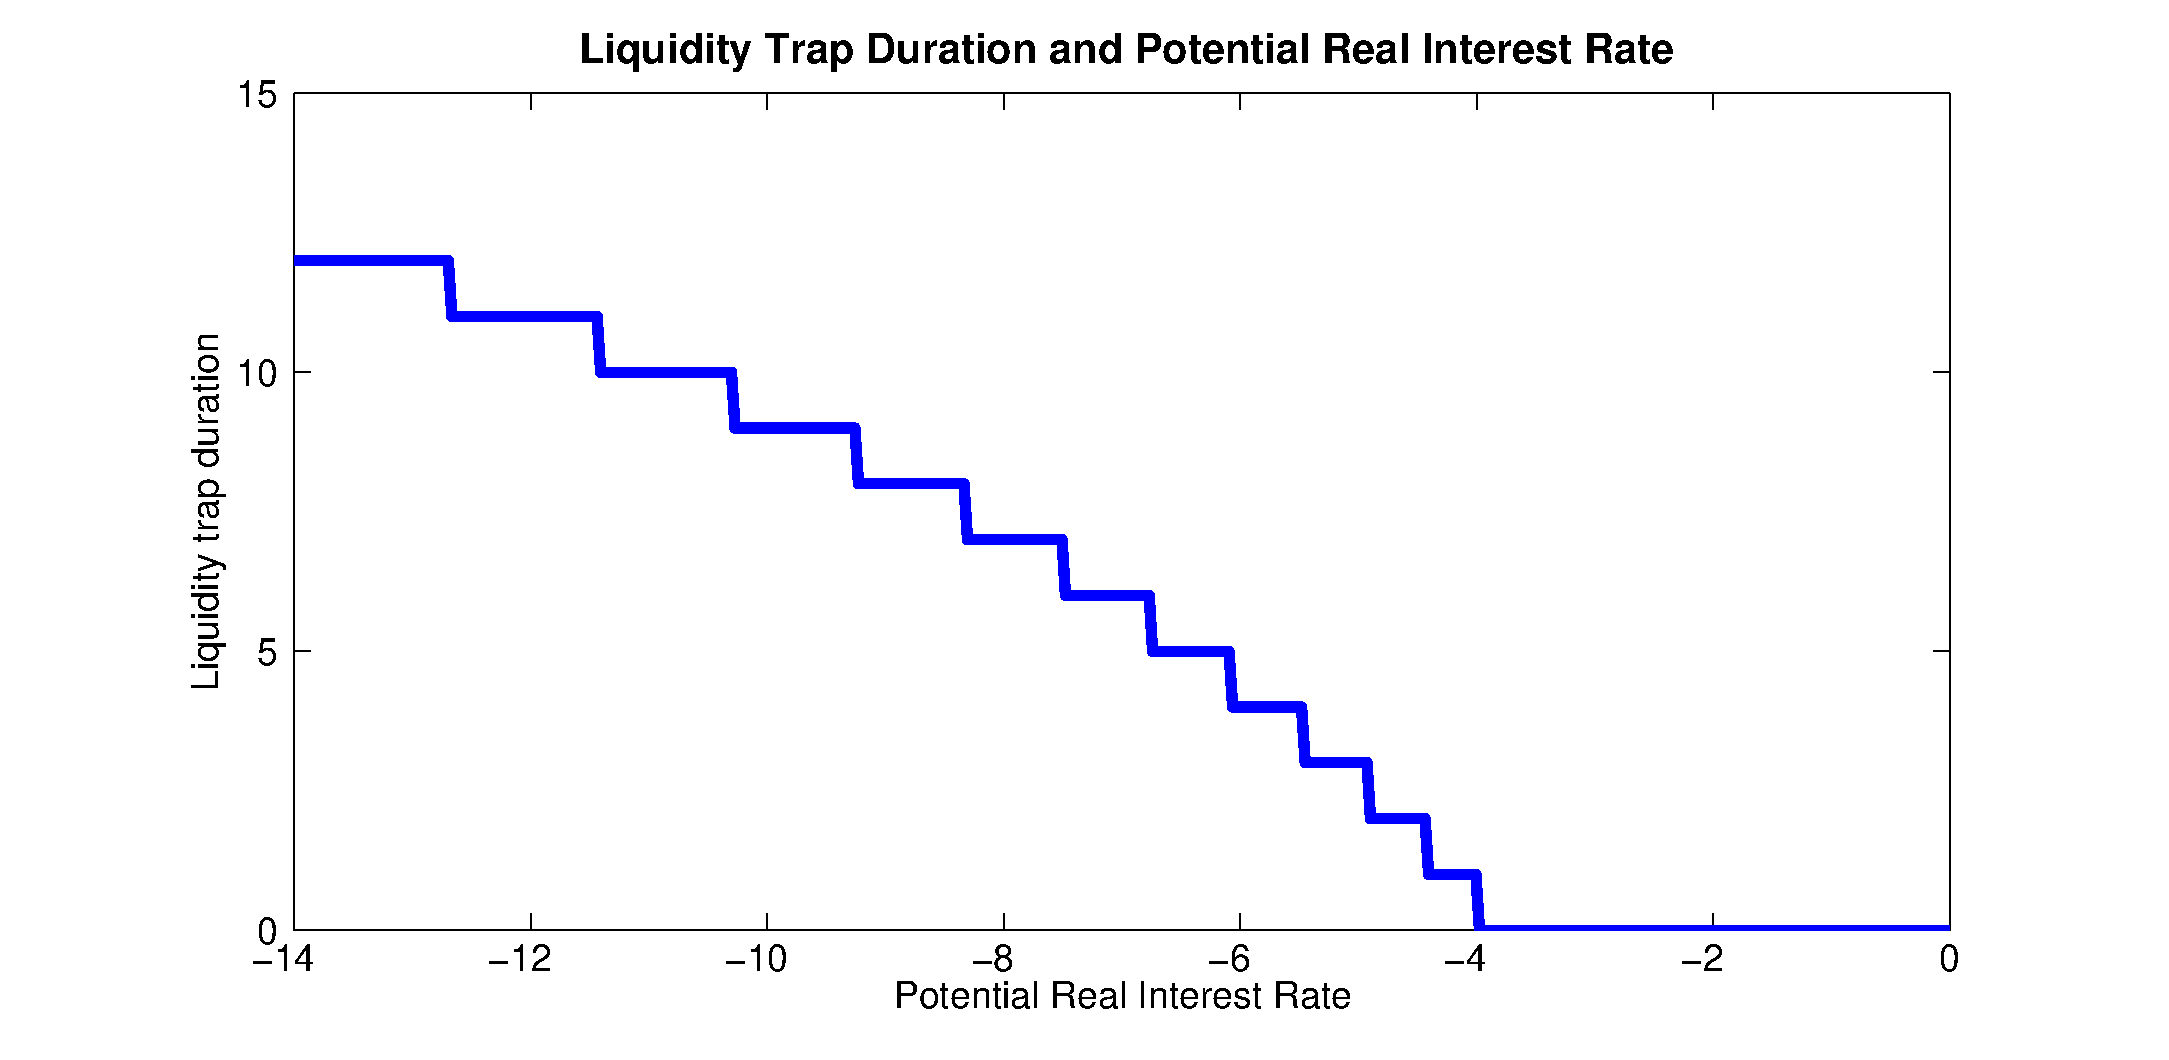
\includegraphics[width=\textwidth]{Paperpics/Figure1b}
\caption{Potential Real Interest Rate and Variation of Taste Shock}
\label{Figure1b}
\end{figure}
\bigskip


\begin{figure}[th]
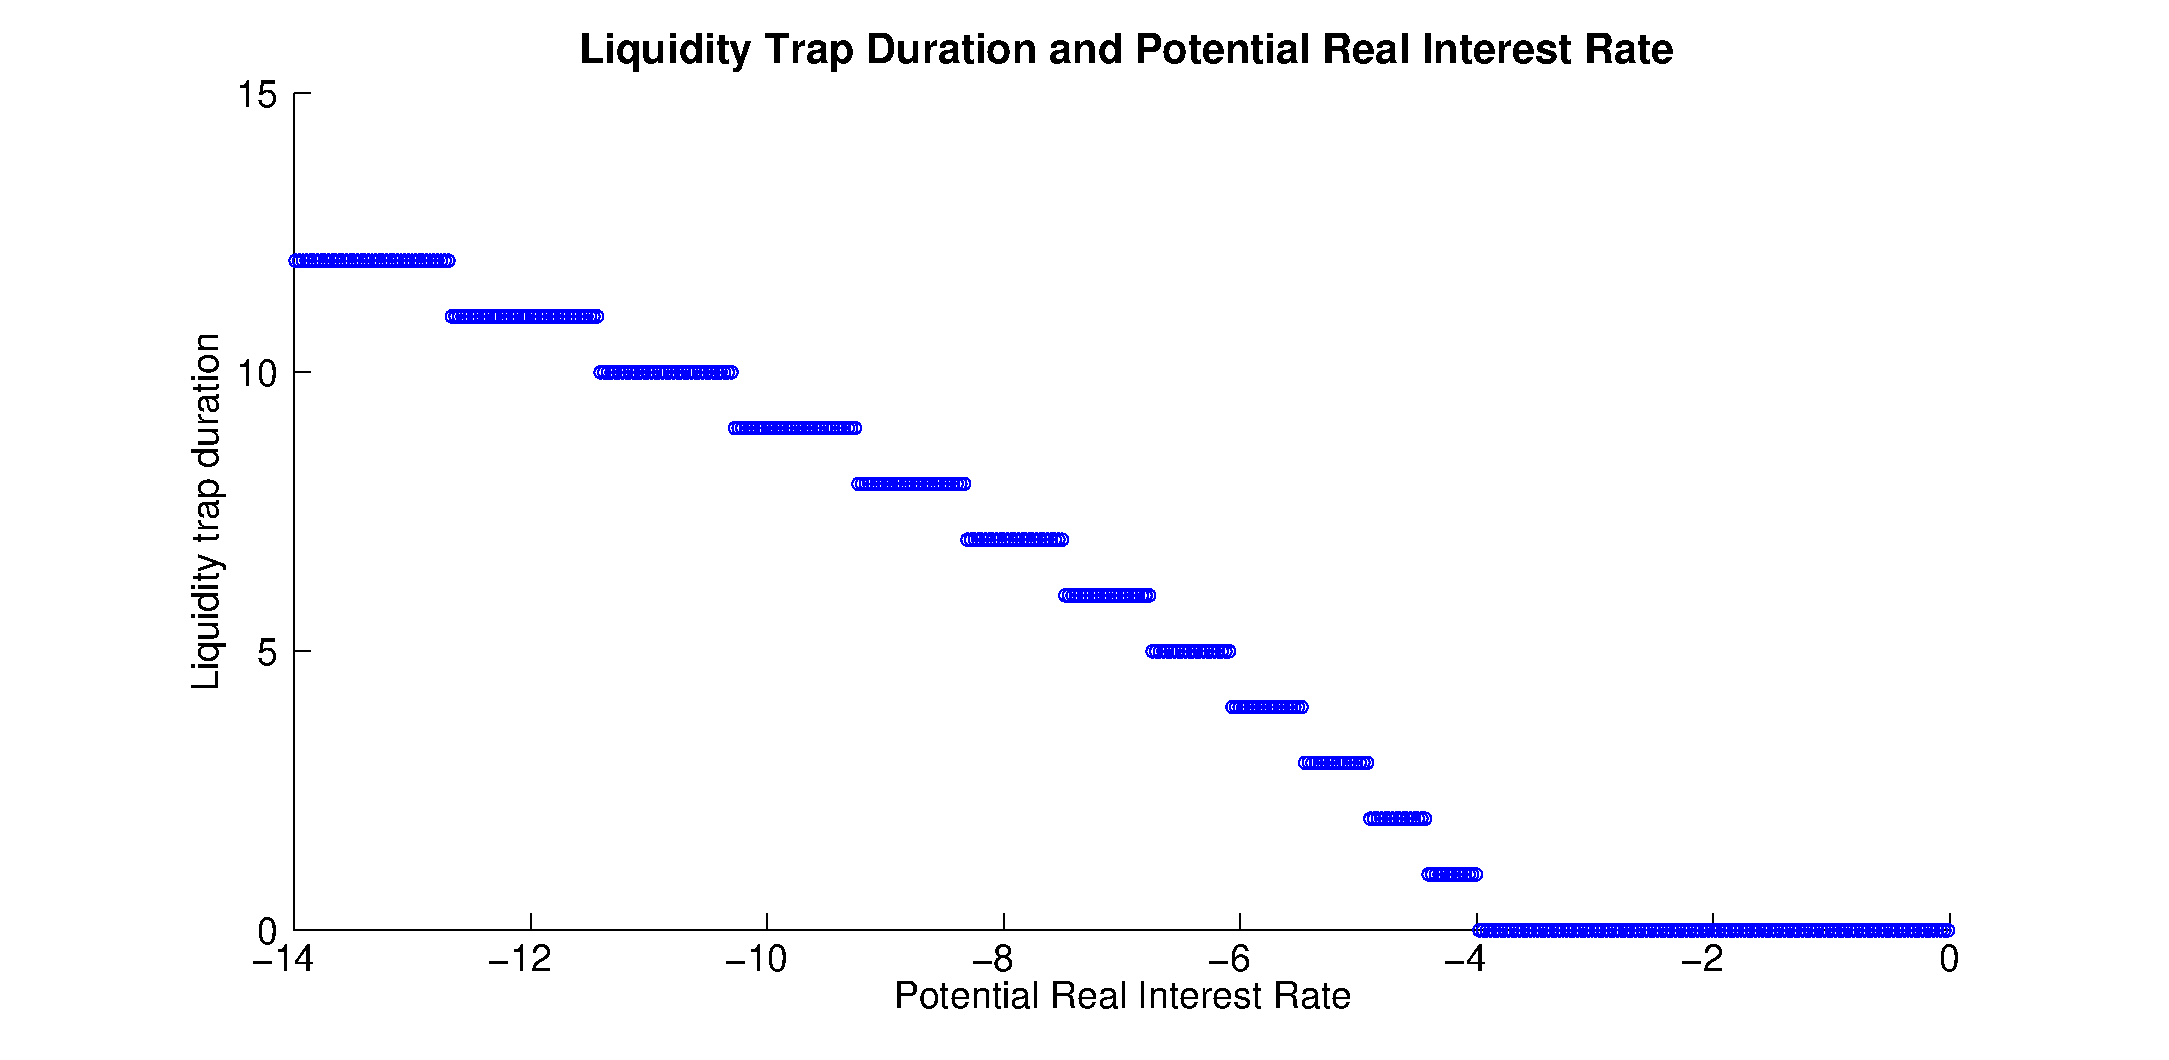
\includegraphics[width=\textwidth]{Paperpics/Figure1bscatter}
\caption{Potential Real Interest Rate and Variation of Taste Shock (Scatter plot)}
\label{Figure1bscatter}
\end{figure}
\bigskip

% \begin{figure}[th]
% \includegraphics[width=\textwidth]{Paperpics/}
% \caption{Spending Multiplier in a simple New Keynesian Model (No Inflation Response)}
% \label{GSMnoinflation}
% \end{figure}
% \bigskip
%
% \begin{figure}[th]
% \includegraphics[width=\textwidth]{Paperpics/}
% \caption{Multiplier Schedule: Implications to Y and G}
% \label{MultiplierSchedule}
% \end{figure}
% \bigskip
%
% \begin{figure}[th]
% \includegraphics[width=\textwidth]{Paperpics/}
% \caption{Spending Multiplier in a simple New Keynesian Model (Alternative Price Contract Duration)}
% \label{GSMalternativeprices}
% \end{figure}
% \bigskip
%
% \begin{figure}[th]
% \includegraphics[width=\textwidth]{Paperpics/}
% \caption{Government Debt Response in a simple New Keynesian Model (No Inflation Response)}
% \label{GovernmentDebtnoinflation}
% \end{figure}
% \bigskip
%
% \begin{figure}[th]
% \includegraphics[width=\textwidth]{Paperpics/}
% \caption{Government Debt Response in a simple New Keynesian Model (Alternative Price Contract Duration}
% \label{GovernmentDebtalternativeprices}
% \end{figure}
% \bigskip



%Tabellen
\newpage

\begin{table}[th]
\centering
\caption{Parameter Values Benchmark Calibration}
\bigskip
\bgroup
\def\arraystretch{1.5}
\begin{tabular}{p{1.2cm} l c}
\toprule\toprule \noalign{\smallskip}
 & \multicolumn{1}{c}{\textit{Description}} & \textit{Value} \\
\hline\noalign{\smallskip}

$\alpha$ & Capital Share   & 0.3 \\
$\beta$  & Discount Factor & 0.995 \\
$\sigma$ & Intertemporal Substitution Elasticity & 1 \\
$\chi$ & Inverse of Frisch-Elasticity & 2.5 \\
$g_c$ & Government Share on Output & 0.2 \\
$\varphi_b$ & Tax Rule Parameter & 0.01 \\
$\nu_c$ & Scale Parameter on the Taste Shock & 0.01 \\
$\rho$ & AR(1) Natural Rate for both Shocks & 0.1 \\
$\xi_p$ & Calvo Parameter (No Inflation) & 1 \\
 & Calvo Parameter (10 quarter price contracts) & 0.9 \\
 & Calvo Parameter (5  quarter price contracts) & 0.8 \\
 & Calvo Parameter (4  quarter price contracts) & 0.75 \\
 & Calvo Parameter (3  quarter price contracts) & 0.667 \\
$\gamma_{\pi}$ & Taylor Rule Coefficient on Inflation & 66.15 \\
$\gamma_x$ & Taylor Rule Coefficient on Output Gap & 66.15 \\
\bottomrule
\end{tabular}
\egroup
\end{table}


\end{document}
